\documentclass{article}
\usepackage{graphicx}
\usepackage{indentfirst}
\usepackage{parskip}
\usepackage{changepage}
\usepackage{hyperref}
\usepackage{titlesec}
\usepackage[backend=biber, style=numeric, citestyle=ieee]{biblatex}
\usepackage{tabularx}
\usepackage[table]{xcolor}
\usepackage{forloop}
\usepackage{longtable}
\newcounter{loopcntr}
\newcommand{\rpt}[2][1]{ \forloop{loopcntr}{0}{\value{loopcntr}<#1}{#2} }
\newcommand{\on}[1][1]{\forloop{loopcntr}{0}{\value{loopcntr}<#1}{&\cellcolor{gray}}}
\newcommand{\off}[1][1]{\forloop{loopcntr}{0}{\value{loopcntr}<#1}{&}}

\newenvironment{subs}
  {\adjustwidth{3em}{0pt}}
  {\endadjustwidth}

\titleformat*{\section}{\small\bfseries}
\titleformat*{\subsection}{\small\bfseries}
\titleformat*{\subsubsection}{\small\bfseries}
\titleformat*{\paragraph}{\small\bfseries}
\titleformat*{\subparagraph}{\small\bfseries}


\addbibresource{references.bib}
\begin{document}

\title{\textbf{A Multi-Swarm Particle Swarm Optimization Solution for the University Course Timetabling Problem}}
\author{Gian Myrl D. Renomeron\\
    CMSC 199.1: Research in Computer Science I\\
    Division of Natural Sciences and Mathematics\\
    University of the Philippines Tacloban College\\
    {\small \href{mailto:gdrenomeron@up.edu.ph}{gdrenomeron@up.edu.ph}}
}
\date{}

\maketitle
\pagebreak
    \section*{A Multi-Swarm Particle Swarm Optimization Solution for the University Course Timetabling Problem}

\section{Introduction}
\label{sec:introduction}

Academic institutions face the significant challenge of efficient resource management in their administrations without compromising the quality of the educational experience in this dynamic world of academia. \cite{Zhang2014-ak} Among the most complicated logistical problems that universities encounter is the so-called \textit{University Course Timetabling Problem} (UCTP). \cite{Arratia-Martinez2021-io} \cite{Oswald_C2013-zo} Essentially, the scheduling of courses, instructors, and students into particular time slots and rooms will match a variety of constraints, including room capacities, faculty availability, and course prerequisites, among others. \cite{Torres2021-ir} It is quite a challenging task to prepare the perfect schedule, especially for larger institutions where manual methods often result in conflicts and inefficiencies. \cite{Arratia-Martinez2021-io}

Latest advanced computational approaches emerged to address these problems, and among them \textit{Swarm Intelligence} (SI) is one of the most promising directions. \cite{Algethami2021-mm} Among the algorithms of this group, there is an attention-grabber - \textit{Particle Swarm Optimization} (PSO) \cite{kennedy1995particle}, distinguished by adaptability and efficiency in searching large solution spaces. \cite{Chen2013-cp} \cite{Ali2014-mb} The algorithm is represented by a set of particles, which are possible solutions; each particle moves in the search space, and its position changes according to individual and collective experiences. \cite{Gunawan2008-ga} Still, despite many strengths, PSO fails at times to solve problems efficiently within UCTP, often failing to find the best solution under tight constraints. \cite{Oswald_C2013-zo}

Multi-Swarm Optimization (MSO) is designed to split up the main swarm into smaller, specialized sub-swarms that concurrently operate in exploiting different regions of the solution space simultaneously. \cite{Bacanin2022-multiswarm} It aims to improve the capabilities of PSO by focusing on issues such as search diversity and the global optimizing ability of the algorithm. \cite{XIA2018126} One of such particular modifications of the above-mentioned technique is MSPSO: \textit{Multi-Swarm Particle Swarm Optimization}, which dynamically varies the sub-swarms in the standard PSO in both exploration and exploitation for a good performance to provide capabilities of global and local search. \cite{XIA2018126} To make this approach balanced, mechanisms for exploration and exploitation are integrated appropriately such that different solution domains would be explored in detail while optimizing the potential solutions in a balanced manner. \cite{Wang2023-ps} 

This paper introduces a new approach to solving the UCTP based on multi-swarm PSO only. MSPSO is specially designed for university course timetabling with diverse constraints, while search methods are efficient in finding optimal timetables. This approach promises to provide schedules that are conflict-free as well as resource-efficient and meet the specific needs of educational institutions. This effort aims to contribute towards scalable and realistic automation and optimization of timetabling, responding to one of the most complex problems in academic administration.


\begin{subs}
\subsection{Background of the Study}
\label{subsec:background}
\begin{itemize}
    \item[] \textbf{University Course Timetabling Problem (UCTP)}
    
    The \textit{University Course Timetabling Problem} (UCTP) is defined as a problem of making assignments for courses, instructors, and students to particular time slots and rooms according to numerous constraints, for example room capacities and instructor availability.\cite{Zhang2014-ak} \cite{Oswald_C2013-zo} \cite{Chen2013-cp} UCTP is a classic problem of academic optimization, and quality methods are demanded for efficient scheduling.\cite{Arratia-Martinez2021-io} \cite{Lih2018-km} \cite{Yang2017-ly} 

    \item[] \textbf{Swarm Intelligence}
    
    \textit{Swarm Intelligence} refers to bio-inspired algorithms based on the collective behavior of animals such as ants, bees, or birds. \cite{Gao2024-apso} \cite{Fallahi2022-qpso} It is applied to optimization problems because it can efficiently and adaptively search very large solution spaces. \cite{Oswald_C2013-zo} \cite{Gao2024-apso}

    \item[] \textbf{Particle Swarm Optimization (PSO)}
    
    \textit{Particle Swarm Optimization (PSO)} is the best known among SI algorithms. \cite{Liu2017-clqpso} It simulates the motions of particles, which denote solutions, in the search space and updates them based on individual and collective experiences. \cite{kennedy1995particle} \cite{Ali2014-mb} \cite{Zhan2009-apso} PSO performs very well on many optimization problems, such as UCTP, but still struggles with tricky constraints. \cite{Oswald_C2013-zo} \cite{Chen2013-cp} 

    \item[] \textbf{Multi-Swarm Optimization (MSO)} 

    \textit{Multi-Swarm Optimization (MSO)} is an advanced extension of swarm intelligence algorithms. \cite{blackwell2004multi} The basic idea in MSO is to divide the primal swarm into multiple sub-swarms that scan concurrently the different areas of the solution space. A concurrent search makes the algorithm have a better opportunity to discover global optima with effective balancing between exploration and exploitation. \cite{Bacanin2022-multiswarm}.

    \item[] \textbf{Multi-Swarm Particle Swarm Optimization (MSPSO)} 
    
    \textit{Multi-Swarm Particle Swarm Optimization (MSPSO)} is a PSO algorithm developed to overcome the lack of diversity of search and local optima avoidance in the process of complex optimization problems, by splitting the main swarm into a considerable number of subswarms that explore different regions in parallel with the solution space, hence, it promotes diversity and the likelihood of finding the global optima. \cite{blackwell2004multi} The difference gives the algorithm an excellent improvement in searching for such solutions for complex problems, such as the UCTP, which balanced exploration and exploitation would provide. \cite{XIA2018126} \cite{Liu2023-pso} 

\end{itemize}

\subsection{Related Works}
\label{subsec:relatedworks}

In the field of UCTP, metaheuristic approaches have been studied for extensive potential towards providing valid and effective solutions with respect to constraints. Metaheuristics aim at establishing quick but effective solutions by approximating optimal schedules rather than executing exhaustive searches, which can sometimes be very computationally expensive.

A two-stage very popular heuristic strategy by Bong Chia Lih et al. \cite{Lih2018-km} gives the first stage to be the grouping of all courses that can be held at the same time, and the second stage to be the assignment of time slots and venues for these groups. Meanwhile, the approach lowers the complexity of this problem, and it has already been successfully applied using real university data and it can handle real-world constraints very efficiently. Similar to Zhang et al., \cite{Zhang2014-ak} an efficient greedy heuristic algorithm handles room and time-slot assignments. Thus, the presented approach, emphasizing the predefined constraints, can meet the required flexibility by these timetables and institutional requirements.

Further, Yanming Yang et al. \cite{Yang2017-ly} proposed a genetic algorithm with self-adaptive crossover and mutation probabilities, which along with a preservation strategy, led to optimal schedules. Although technically in the category of genetic algorithms, a technique based on adaptive nature is close to metaheuristic techniques and thus highly efficient for timetabling in dynamic environments such as military academies. Alves et al. \cite{Alves2018-ar} further enhanced the genetic approach by developing a recursive GA that maximizes efficiency in course timetabling when real-world constraints and evolving scheduling demands are considered.

Other metaheuristic methods applied in solving UCTP include Particle Swarm Optimization (PSO). PSO is another optimization technique that is increasingly gaining acceptance in solving UCTP problems. The concept was derived from the social behavior a swarm of birds or of fish follows. This makes it possible to adopt the efficient exploration of large search spaces. Oswald and Durai \cite{Oswald_C2013-zo} proposed a hybrid PSO with strategies for improving search applied particularly for UCTP. This was well balanced between exploration and exploitation so the robust timetabling solutions in reference to Oswald et al 2013. Similarly, Chen and Shih \cite{Chen2013-cp} created a constriction PSO model integrated with local search strategies to enhance both the gain in generation speed of solutions and the quality of the solution obtained. It has shown the effectiveness of PSO in solving challenging scheduling problems.

Generalizing the metaheuristic methods embraced here, such as greedy algorithms, adaptive genetic strategies, and PSO-based techniques, indicate that these are feasible for solving UCTP. In fact, these methods are not a global optimality guarantee; however, speed and flexibility in an ideally minimal number of computations make them highly valuable tools for educational institutions, especially for large-scale tasks where a large number of constraints are to be balanced.

\end{subs}


\section{Statement of the Problem}
\label{sec:problemstatement}

The UCTP problem is quite complex and key for any institution of learning because it considers assigning courses to specific rooms and time slots while considering constraints such as room capacities, course prerequisites, and faculty courses. \cite{Arratia-Martinez2021-io} To this date, most universities still consider non-optimal manual or heuristic methods, and the inefficiencies include uneven teaching loads and a mismatch between qualifications and requirements in course teaching. \cite{Oswald_C2013-zo} \cite{Gunawan2008-ga} While the complexity of the problem is increased, it happens to be highly infeasible to find the best solutions, especially when there are conflicting constraints that need to be fulfilled. 

The existing work \cite{Oswald_C2013-zo} \cite{Ali2014-mb} \cite{Chen2013-cp} used PSO-based techniques in solving UCTP but highly developed approaches are required to be found due to the complexity of the problem, such as MSPSO, this improves the original PSO technique by splitting the swarm into many sub-swarms that simultaneously start exploring different regions of solution space. This allows for a higher degree of diversity in search and avoids getting trapped in the local optimum for a better possibility of finding the global optimum.

This paper focuses on the development of a solution for UCTP using MSPSO, that is, to explore the vast solution space with much greater efficiency than before, paying attention to constraints like room capacities, course prerequisites, and scheduling conflicts. In terms of metrics like balance of workloads, course-faculty alignment, and computational efficiency, this proposed approach is supposed to bring about improvements in quality and fairness in the courses scheduled within institutions.

\section{Objectives of the Study}
\label{sec:objectives}

\subsection{General Objective}
\label{subsec:generalobjective}

To design and develop a Multi-Swarm Particle Swarm Optimization (MSPSO) algorithm to solve the University Course Timetabling Problem (UCTP).

\subsection{Specific Objectives}
\label{subsec:specificobjectives}
\begin{enumerate}
    \item To examine how the MSPSO algorithm is used and how well it solves the UCTP. 
    \item To model the UCTP with crucial characteristics like room availability, course prerequisites, and faculty courses within the framework of MSPSO. 
    \item To perform a state-of-the-art analysis by contrasting the MSPSO approach with current techniques used in the UCTP 
    \item To deploy a web-based application that uses the MSPSO approach for generating university course timetabling.
\end{enumerate}

\section{Scope and Limitation}
\label{sec:scopeandlimitation}

In the context of solving the UCTP problem, the focus is on the implementation of the MSPSO algorithm. The study will execute its experiment using the data instance of a particular UCTP, thereby limiting its generalizability to different timetabling scenarios, not necessarily on the exact data set. It does not include dynamic factors that may unexpectedly appear in the scheduling stage. Examples of such factors include the alteration of course schedule at the last minute and sudden availability of rooms. Other optimization models aside from the MSPSO used in the study were not included along with hybrid approaches. This is how the scope of the present research was set, and opportunities were presented for further consideration and adaptation to other school settings.

\section{Significance of the Study}
\label{sec:significance}

The importance of this paper is developing a new approach for solving the University Course Timetabling Problem using Multi-Swarm Particle Swarm Optimization. To be more specific, because numerous methods have been widely applied to solve UCTP, MSPSO is the first approach that explores more extensive areas of solutions through the use of more than one sub-swarm. This new technique aims to generate high-quality, conflict-free timetables that respect necessary constraints such as room capacities, course prerequisites, and faculty schedules, thereby advancing the field of university scheduling.

Besides the academic value, this research opens up possibilities for wider applications of MSPSO in fields requiring efficient scheduling and resource management. With the establishment of MSPSO as an efficient strategy for UCTP, this study opens avenues for its use in other complex scheduling scenarios related to healthcare, transportation, and manufacturing. These contexts are critical where optimum planning and resource utilization must occur. The research outcomes from this study might stimulate new studies and further applications in MSPSO for diverse industry fields.

Therefore, this paper not only develops a novel solution for scheduling at the university level but also lays down a foundation that may help in further studying MSPSO as a broad tool for automated scheduling in multiple industries.

\section{Theoretical and Conceptual Framework}
\label{sec:theoreticalframework}

\begin{figure}[h] % h stands for 'here'
    \centering
    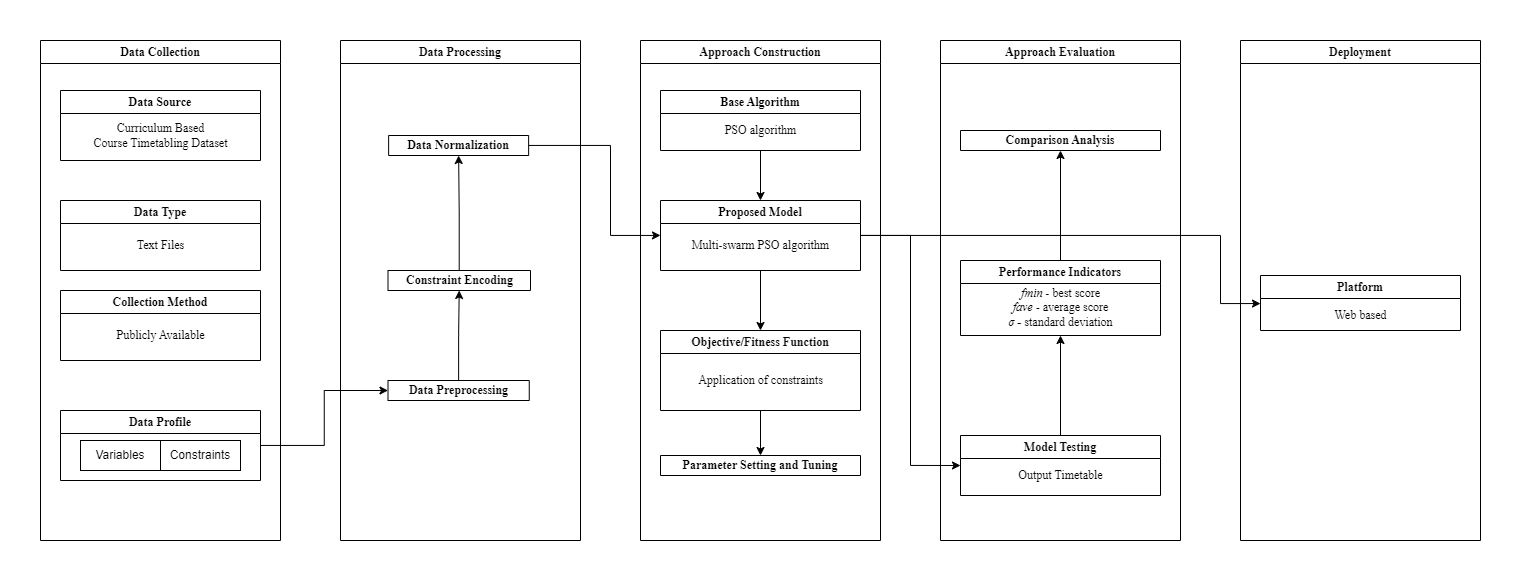
\includegraphics[width=1\textwidth]{framework}
    \caption{Theoretical and Conceptual Framework}
    \label{fig:framework} % label for referencing
\end{figure}

The theoretical and conceptual framework of this study consists of five separate yet connected components: Data Collection, Data Processing, Approach Construction, Approach Evaluation, and Deployment. The workflow starts with the Data Collection phase, collecting benchmark datasets and optimization problem instances. These datasets usually are publicly available and typically represented in text or XML formats. This phase ensures that there is adequate sourcing and data variety to support the solid analysis of the optimization model against different conditions. Steps undertaken in the Data Processing step include cleaning the data to remove inconsistencies and make sure that all inconsistencies in constraints are encoded in apt forms of mathematics for solving before preparing the data for optimized use. Data cleaning removes errors or missing values that could have otherwise affected the model's performance while encoding constraints take problem-specific rules and transform them into a format that could be used by the model. Normalization and data categorization are also considered uniform since the optimization model can cope well with the data. All these processes, therefore, collectively provide standardized and reliable input for the optimization phase. This ensures that the information is valid and appropriate to the model in question. It will act as a foundation for later phases.

The construction of the approach deals with the creation of the model of multi-swarm optimization. This acts as a core method for the optimization problem solution. A part of this component deals with the base model setup and setting parameters that make the model capable of appropriately addressing the needs of the problem. The Approach Evaluation phase involves testing the performance of the model based on whether it satisfies any required objectives. This phase must be done to determine how well the proposed model is and make adjustments according to what is needed to increase its applicability. Lastly, the solution would be deployed by presenting an optimized solution via the use of a web-based interface, where users will have the ability to upload their problem instances and find real-time optimized outputs for their respective problems. All parts are included to be effective contributors to the solution development process, ensuring that data is handled properly, models built and evaluated appropriately, and the final solution is practically deployable. 

\subsection{Concepts, Theories, and Methodologies Reused}

This paper employs current swarm intelligence theories and algorithms, mainly in Particle Swarm Optimization (PSO) \cite{kennedy1995particle} and Multi-Swarm Optimization (MSO) \cite{blackwell2004multi}. PSO is an established algorithm to efficiently search large solution spaces by a set of particles that are exploring a search area with individual and collective experiences. Parsopoulos and Vrahatis \cite{parsopoulos2002recent} first introduced neighborhood-based swarming in global and local variants in the introduction of the MSO approach. That paper set a solid basis for multi-swarm frameworks. The structure of the neighborhood and dynamic tuning of parameters discussed there provided important inspirations for later developments in multi-swarm optimization. One of the first spectacular applications of these multi-swarm approaches is given by Blackwell and Branke \cite{blackwell2004multi}, who studied MSO in dynamic settings. These methodologies are crucial to establish the foundation for MSPSO.

\subsection{Concepts, Theories, and Methodologies Modified}

To improve existing PSO and MSO methodologies, the research here modifies the base methodologies to take on a multi-swarm structure particularly designed for UCTP, called MSPSO. The MSPSO algorithm divides the main swarm into smaller, specialized sub-swarms operating in parallel to explore the solution space more effectively at different parts. \cite{XIA2018126} \cite{blackwell2004multi} THe improvement is designed to circumvent the limitations of lack of search diversity and trapping into local optima through the encouragement of a greater exploration of solution possibilities along with the exploitation of promising regions. The modification improves better adaptability and efficiency in generating feasible course timetables.

\subsection{Novel Concepts, Theories, and Methodologies Introduced}

This research introduces a new optimization approach for UCTP via MSPSO, specifically designed to address complex timetabling constraints such as room availability, faculty preferences, and scheduling conflicts. Its novelty lies in the combination of dynamic swarm partitioning and targeted exploration, allowing the MSPSO algorithm to achieve workload balance and enhance resource use within educational institutions \cite{Bacanin2022-multiswarm}. The proposed MSPSO-based methodology balances mechanisms for exploration and exploitation, ensuring that the different solution domains are discovered thoroughly to allow the provision of optimal scheduling solutions.

\section{Methodology}
\label{sec
}

This section outlines the methodology of using MSPSO to effectively solve the UCTP.

\subsection{Data Collection}
\label{subsec} 
\begin{itemize} \item Decompose the UCTP into exploratory and refinement components. \item Identify exploratory tasks suitable for MSPSO and refinement tasks for IP. \item Define the structure of the solutions represented by particles in MSPSO, including course, room, and time slot assignments. \end{itemize}


\subsection{Data Processing}
\label{subsec}


\subsection{Approach Construction}
\label{subsec
} \begin{itemize} \item Initialize multiple swarms to explore various potential timetabling solutions. \item Define the representation of solutions (particle encoding) for the assignment of courses to rooms and time slots. \item Develop a fitness function to evaluate solutions based on: \begin{itemize} \item Minimizing scheduling conflicts (e.g., room clashes, instructor availability). \item Maximizing resource usage (e.g., optimal room utilization and course distribution across time slots). \end{itemize} \item Implement the MSPSO algorithm: \begin{itemize} \item Update particle positions and velocities based on individual and global best solutions. \item Perform iterations until a convergence criterion is met or a predefined number of iterations is reached. \item Collect the best solutions generated by the swarms for refinement. \end{itemize} \end{itemize}

\subsection{Approach Evaluation}
\label{subsec
} \begin{itemize} \item Post-process the final timetabling solutions to evaluate against key performance metrics: \begin{itemize} \item Conflict minimization: Ensure no room or instructor conflicts in the final schedule. \item Course-resource alignment: Maximize the alignment of course scheduling with available room resources and time slots. \item Computational efficiency: Measure the overall performance of the hybrid optimization approach in terms of speed and accuracy. \end{itemize} \item Select the best overall timetable based on the combination of fitness and objective evaluations. 
\end{itemize}

\subsection{Deployment}

\section{Schedule of Activities}
\label{sec:schedule}

\begin{longtable}{| p{0.18\textwidth} | p{0.18\textwidth} | p{0.18\textwidth}*{12}{|p{0.01\textwidth} }| }
    \hline
    \textbf{OBJECTIVES} & \textbf{TARGET ACTIVITIES} & \textbf{TARGET ACCOMPLISHMENTS} (quantify, if possible) & \multicolumn{12}{|c|}{\textbf{YEAR 1}} \\
    \hline
     & & & 1 & 2 & 3 & 4 & 5 & 6 & 7 & 8 & 9 & 10 & 11 & 12 \\
    \hline
    Objective 1 & 
        To examine how the MSPSO algorithm is used and how well it solves the UCTP. & 
    1. Gather relevant literature on MSPSO applications.\newline 
    2. Analyze the performance of MSPSO on test datasets.\newline
    3. Evaluate the effectiveness of MSPSO in solving UCTP with various constraints.
        \off[8] \on[4] \\ 
    \hline
    Objective 2 & 
        To model the UCTP with crucial characteristics like room availability, course prerequisites, and faculty courses within the framework of MSPSO. & 
    1. Identify and define critical constraints in UCTP.\newline 
    2. Develop and model UCTP using MSPSO framework.\newline
    3. Test the model on synthetic and real data.
        \off[9] \on[3] \\ 
    \hline
    Objective 3 & 
        To perform a state-of-the-art analysis by contrasting the MSPSO approach with current techniques used in the UCTP. & 
    1. Benchmark MSPSO against other UCTP methods like GA and PSO.\newline 
    2. Conduct performance evaluations and analysis.
        \off[11] \on[1]  \\ 
    \hline
\end{longtable}

\begin{longtable}{| p{0.18\textwidth} | p{0.18\textwidth} | p{0.18\textwidth}*{12}{|p{0.01\textwidth} }| }
    \hline
    \textbf{OBJECTIVES} & \textbf{TARGET ACTIVITIES} & \textbf{TARGET ACCOMPLISHMENTS} (quantify, if possible) & \multicolumn{12}{|c|}{\textbf{YEAR 2}} \\
    \hline
     & & & 1 & 2 & 3 & 4 & 5 & 6 & 7 & 8 & 9 & 10 & 11 & 12 \\
    \hline
    Objective 3 & 
        To perform a state-of-the-art analysis by contrasting the MSPSO approach with current techniques used in the UCTP. & 
    1. Conduct a detailed analysis and comparison with existing UCTP techniques.\newline 
    2. Publish results and make recommendations for improvements.
        \on[5] \off[7] \\ 
    \hline
\end{longtable}

\printbibliography 
\end{document}